% This is samplepaper.tex, a sample chapter demonstrating the
% LLNCS macro package for Springer Computer Science proceedings;
% Version 2.21 of 2022/01/12
%
\documentclass[runningheads]{llncs}
%
\usepackage[T1]{fontenc}
% T1 fonts will be used to generate the final print and online PDFs,
% so please use T1 fonts in your manuscript whenever possible.
% Other font encondings may result in incorrect characters.
%
\usepackage{graphicx}
% Used for displaying a sample figure. If possible, figure files should
% be included in EPS format.
%
% If you use the hyperref package, please uncomment the following two lines
% to display URLs in blue roman font according to Springer's eBook style:
%\usepackage{color}
%\renewcommand\UrlFont{\color{blue}\rmfamily}
%\urlstyle{rm}
%
\usepackage{tikz}
\usetikzlibrary{shapes.geometric, arrows.meta, positioning}
\tikzstyle{process} = [rectangle, minimum width=0.8cm, minimum height=0.2cm, text centered, draw=black, fill=gray!10, font=\bfseries]
\tikzstyle{arrow} = [thick, -{Stealth[length=3mm]}]

\begin{document}
%
\title{Virtual Humans for HCI: A Design Framework for Adaptive Multimodal Agents }

\titlerunning{Virtual Humans for HCI}
% If the paper title is too long for the running head, you can set
% an abbreviated paper title here
%
\author{Tarun Shyam Ravi}
%
\authorrunning{Tarun Shyam Ravi}
% First names are abbreviated in the running head.
% If there are more than two authors, 'et al.' is used.
%
\institute{Brandenburgische Technische Universität Cottbus-Senftenberg
\\email{: shyamtar@b-tu.de}\\
\url{https://www.b-tu.de/}}
%
\maketitle           % typeset the header of the contribution
%
\begin{abstract}
Virtual Humans are becoming a prominent modality in Human-Computer Interaction (HCI), enabling more natural and expressive communication by integrating speech, facial expressions, and embodiment. This paper introduces a multimodal framework for real-time interaction, combining automatic speech recognition (ASR), large language models (LLMs), and text-to-speech (TTS) with a behavior control module for audio-driven facial animation. The behavior model adopts a dual-stream architecture that processes articulatory and prosodic features independently before fusing them to produce temporally aligned, continuous blendshape-based facial movements. By capturing both the linguistic content and emotional nuance of speech, the system enables synchronized verbal and non-verbal responses via a 3D avatar. The proposed design advances the realism and coherence of virtual human agents, contributing to the broader development of embodied AI and affective computing.
\keywords{Virtual Humans \and Interactive AI \and Adaptive Systems}
\end{abstract}

\section{Introduction}

Human-Computer Interaction (HCI) has evolved from command-line and graphical interfaces to more recent developments in conversational agents. Despite this progress, many of these systems remain limited in their ability to convey non-verbal cues—an essential component of natural human communication. To bridge this gap, \textit{Virtual Humans}—embodied agents with human-like facial features and behavior—are being explored as a means of enabling richer, more intuitive interaction.

This paper presents a framework for Virtual Humans that integrates speech recognition, language modeling, and 3D facial animation using blendshapes. The animation is driven by a facial rig composed of predefined blendshape targets, allowing the avatar to perform nuanced expressions in real time. The system processes user input through a multimodal pipeline and responds with synchronized verbal and non-verbal outputs, including lip movements and gaze behavior. By simulating expressive interaction, the agent aims to enhance engagement, realism, and usability in digital environments.

%\section{Introduction}

%Human-Computer Interaction (HCI) has evolved from command-line and graphical interfaces to more recent developments in conversational agents. Despite this progress, many of these systems remain limited in their ability to convey non-verbal cues—an essential component of natural human communication. To bridge this gap, \textit{Virtual Humans}—embodied agents with human-like facial features and behavior—are being explored as a means of enabling richer, more intuitive interaction.

%This paper presents a framework for Virtual Humans that integrates speech recognition, language modeling, and 3D facial animation using blendshapes. The system processes user input through a multimodal pipeline and responds with synchronized verbal and non-verbal outputs, including lip movements and gaze behavior. By simulating expressive interaction, the agent aims to enhance engagement, realism, and usability in digital environments.

\subsection{Facial Structure and Parametric Control}

A fundamental component of virtual human design is the simulation of facial expressions through a detailed three-dimensional (3D) face model. Contemporary systems often utilize dense facial landmark meshes—such as the 468-point configuration used by MediaPipe Face Mesh—which offer comprehensive coverage of key facial regions, including the lips, eyes, jaw, eyebrows, and forehead. These landmarks enable high-precision tracking and serve as the geometric basis for expressive animation.

Facial movements are commonly encoded using the Facial Action Coding System (FACS), which decomposes expressions into a standardized set of Action Units (AUs). Each AU represents the activation of specific facial muscles—for example, AU01 (inner brow raise), AU04 (brow lower), or AU12 (lip corner pull). These Action Units are then mapped to a set of \textit{blendshapes}—parametric deformations of the 3D mesh that, when weighted and combined, produce dynamic, expressive animations in real time.

\begin{figure}[ht]
\centering
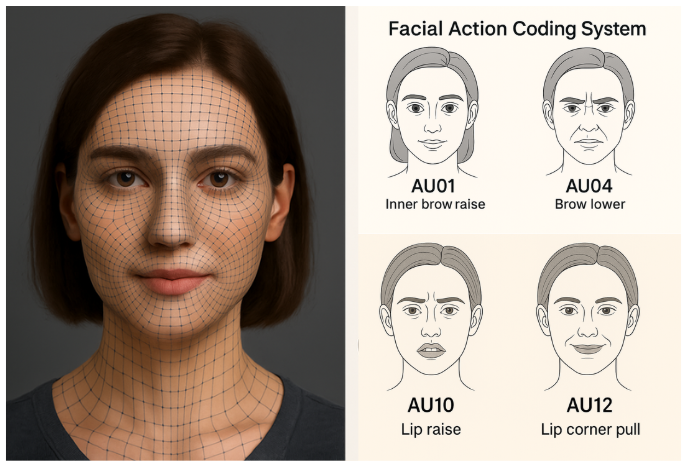
\includegraphics[width=0.8\textwidth]{AU.png}
\caption{Facial Action Coding System (FACS) visualized in a blendshape-based 3D avatar. Each Action Unit (AU) drives a corresponding blendshape, enabling the avatar to render complex expressions in response to speech or emotional context.}
\label{fig:face-animation}
\end{figure}

\subsection{Speech-Driven Expression Through Blendshapes}

During speech, facial regions—especially around the mouth—undergo rapid, phoneme-dependent changes in shape. In Virtual Humans, these articulations are synthesized by driving a set of \textit{blendshapes} that deform specific mesh regions according to the incoming audio signal. Each phoneme is mapped to a corresponding \textit{viseme}, and every viseme is expressed through a weighted combination of blendshape parameters.

As an illustrative example, the vowel sound \textit{AA} (as in \textit{father}) triggers several key deformations: the jaw descends with \textit{JawOpen} set to 0.8; the oral cavity widens via \textit{MouthOpen} at 0.5; the lower lip is pulled downward by \textit{LowerLipDepressor} at 0.7; and lateral expansion is achieved with \textit{MouthStretch} at 0.2. These weights are updated on a frame-by-frame basis, allowing seamless transitions between consecutive visemes and yielding realistic lip-sync.

Because adjacent phonemes influence one another—a phenomenon known as co-articulation—the system continuously interpolates blendshape values rather than switching discretely. This continuous mapping enables the Virtual Human to reproduce speech articulation smoothly and believably, preserving both timing and expressiveness.


\section{Dataset}

To develop and evaluate the speech-driven facial animation system, we utilized a combination of publicly available audiovisual datasets that contain aligned speech and facial expressions. The primary dataset used was the RAVDESS (Ryerson Audio-Visual Database of Emotional Speech and Song), which includes recordings from 24 professional actors delivering both neutral and emotionally expressive speech. Each sample provides synchronized video, audio, and emotion labels, offering a robust basis for modeling both articulation and emotional variance.

Facial deformation data was extracted using MediaPipe Face Mesh, which tracks 468 facial landmarks per frame. These landmarks were then post-processed to estimate blendshape weights representing key mouth and jaw movements. Each audio segment was transformed into a log-Mel spectrogram and temporally aligned with the corresponding sequence of derived blendshape parameters, forming the basis for training the audio-to-blendshape regression model.

To improve articulation accuracy, a small custom dataset was created by manually annotating blendshape weights for specific visemes (e.g., \textit{AA}, \textit{T}, \textit{M}). These samples enabled fine-tuned supervision for critical phoneme-to-viseme mappings. All data was normalized per speaker and downsampled to 30 frames per second to maintain consistency with real-time animation requirements.


\section{Behavior Control}

Behavior control in Virtual Humans refers to the generation of coordinated facial movements that reflect both the phonetic content of speech and the speaker’s emotional expression. In the proposed framework, audio input drives not only accurate lip-sync through blendshape animation but also expressive modulation—capturing prosodic features such as pitch, stress, and intensity. These features influence higher-level facial behaviors, including eyebrow raises, cheek tension, and subtle head gestures.

The system combines low-level acoustic descriptors with learned mappings to blendshape parameters, allowing for the synthesis of real-time, temporally coherent facial animations. This dual-focus design ensures that both linguistic articulation and affective cues are embedded into the visual output. Such synchronization enhances believability and emotional resonance in interactions.

This section outlines the core components of behavior control, including acoustic feature extraction, viseme-to-blendshape conversion, and the training of regression models to predict expressive facial dynamics from speech.

\begin{figure}[ht]
\centering
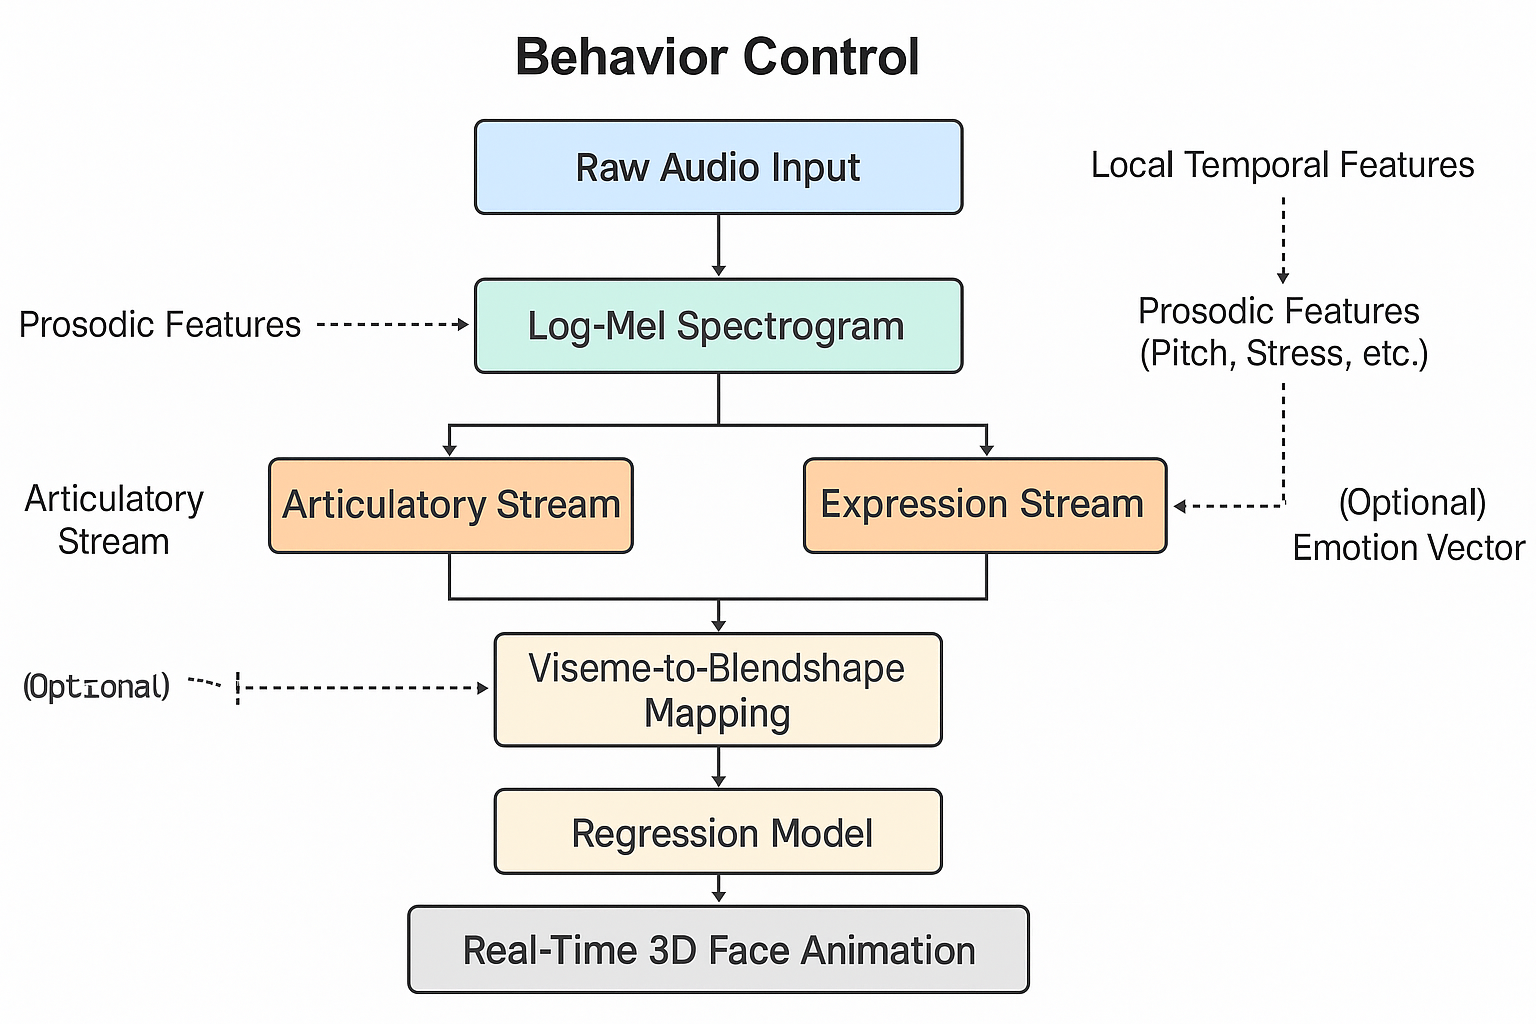
\includegraphics[width=0.85\textwidth]{Be.png}
\caption{1D CNN architecture for audio-to-blendshape regression. Log-Mel features are processed through convolutional layers to capture temporal patterns and are mapped to frame-wise blendshape weights for real-time facial animation.}
\label{fig:model-architecture}
\end{figure}


\subsection{Audio Feature Extraction}

To enable real-time facial animation from speech, the system first transforms raw audio input into structured acoustic features suitable for machine learning. Each audio signal is divided into overlapping frames and converted into a log-Mel spectrogram, which preserves perceptually relevant frequency and temporal information while reducing sensitivity to background noise.

Audio is sampled at 16 kHz and segmented into 25 ms windows with a 10 ms stride. Each frame yields an 80-dimensional log-Mel vector, producing a continuous time-series representation that captures both phonetic content (e.g., vowel and consonant identity) and prosodic cues (e.g., pitch, energy, and speaking rate).

These features serve as input to the blendshape prediction model. Because speech contains information about both articulation (e.g., lip closure for \textit{/m/}) and expression (e.g., vocal stress), the extracted features underpin both verbal and affective aspects of the facial animation.


\subsection{Training and Testing Protocol}

The blendshape prediction model was trained using paired sequences of audio features and ground-truth blendshape weights. The dataset was split into 80\% for training and 20\% for testing, ensuring that speakers were disjoint across the two sets to evaluate generalization.

Training was conducted for 100 epochs with early stopping based on validation loss. The Adam optimizer was used with a learning rate of $1 \times 10^{-4}$. Evaluation metrics included Mean Absolute Error (MAE) and frame-wise correlation between predicted and actual blendshape vectors.

\subsection{Blendshape Prediction}

To generate expressive, time-synchronized facial motion from speech, the system employs a one-dimensional convolutional neural network (1D CNN) that predicts frame-wise blendshape weights from log-Mel audio features. The model processes short, overlapping audio windows to preserve continuity and smooth transitions across time.

The architecture consists of several stacked Conv1D layers, each followed by \textit{ReLU} (Rectified Linear Unit) activations, which introduce non-linearity and support learning complex audio-to-geometry mappings. A final fully connected layer produces a continuous vector of blendshape weights for each frame, corresponding to facial deformations such as jaw drop, lip stretch, and eyebrow raise.

The task is framed as a regression problem to enable smooth, real-valued output. This formulation is crucial for capturing natural coarticulation effects—for instance, the gradual transition from jaw opening for the vowel \textit{AA} to the closure required for \textit{T} or \textit{M}. Unlike classification-based systems, a regression model can represent these intermediate configurations without abrupt shifts.

The network implicitly learns how prosodic elements—such as pitch and energy—modulate the intensity of facial movements. This allows the system to synthesize not only accurate articulation but also emotionally expressive behavior.

Compared to recurrent models such as LSTMs or GRUs, the 1D CNN offers lower inference latency and simpler parallelization, making it suitable for real-time deployment. By training on paired sequences of audio features and target blendshape weights, the network learns to generate continuous, synchronized facial animations aligned with speech. The architecture's receptive field is tuned to capture sub-second dependencies critical for smooth transitions. Additionally, the model generalizes well to unseen speakers due to speaker-independent training and feature normalization.




\subsection{Loss Function and Regularization}

The model is trained using a supervised regression objective that minimizes the difference between predicted and ground-truth blendshape values for each frame. The primary loss function is the \textbf{Mean Absolute Error (MAE)}, also referred to as \textbf{L1 loss}, which is effective for preserving subtle expression variations and is more robust to outliers than Mean Squared Error (MSE). Given a batch of predicted blendshape vectors $\hat{y}$ and ground-truth vectors $y$, the L1 loss is computed as:

\begin{equation}
\mathcal{L}_{\text{L1}} = \frac{1}{N} \sum_{i=1}^{N} \left| y_i - \hat{y}_i \right|
\end{equation}

where $N$ denotes the number of blendshape parameters per frame.

To improve temporal coherence and reduce jitter in the generated animations, a \textbf{temporal smoothness regularization} term is introduced. This term penalizes large fluctuations between consecutive frames and is defined as:

\begin{equation}
\mathcal{L}_{\text{smooth}} = \frac{1}{N - 1} \sum_{i=1}^{N - 1} \left\| \hat{y}_{i+1} - \hat{y}_i \right\|_2^2
\end{equation}

The total loss is a weighted sum of the two components:

\begin{equation}
\mathcal{L}_{\text{total}} = \mathcal{L}_{\text{L1}} + \lambda \cdot \mathcal{L}_{\text{smooth}}
\end{equation}

where $\lambda$ is a regularization coefficient that balances accuracy and smoothness.

To further prevent overfitting and stabilize training, the network includes \textbf{dropout layers} (with rates between 0.3 and 0.5) after each convolutional block, as well as \textbf{batch normalization}. The model is trained using the \textbf{Adam optimizer} with a learning rate of $1 \times 10^{-4}$, and early stopping is employed based on validation loss to avoid overtraining.

This combined approach—L1 regression, temporal smoothing, and architectural regularization—ensures that the resulting facial movements are both perceptually accurate and temporally consistent in real-time deployment scenarios.

\section{Multi-Modal Feature Interaction}

This real-time pipeline forms the perceptual and expressive core of the virtual human architecture. It integrates language understanding, prosodic modeling, and facial animation into a continuous feedback loop, enabling agents to engage users in coherent, emotionally resonant conversations.

\subsection{System-Level Interaction Loop}

The multimodal interaction begins with the user's spoken input and progresses through five core modules, each contributing to the perception or expression of the virtual human:

\begin{figure}[ht]
\centering
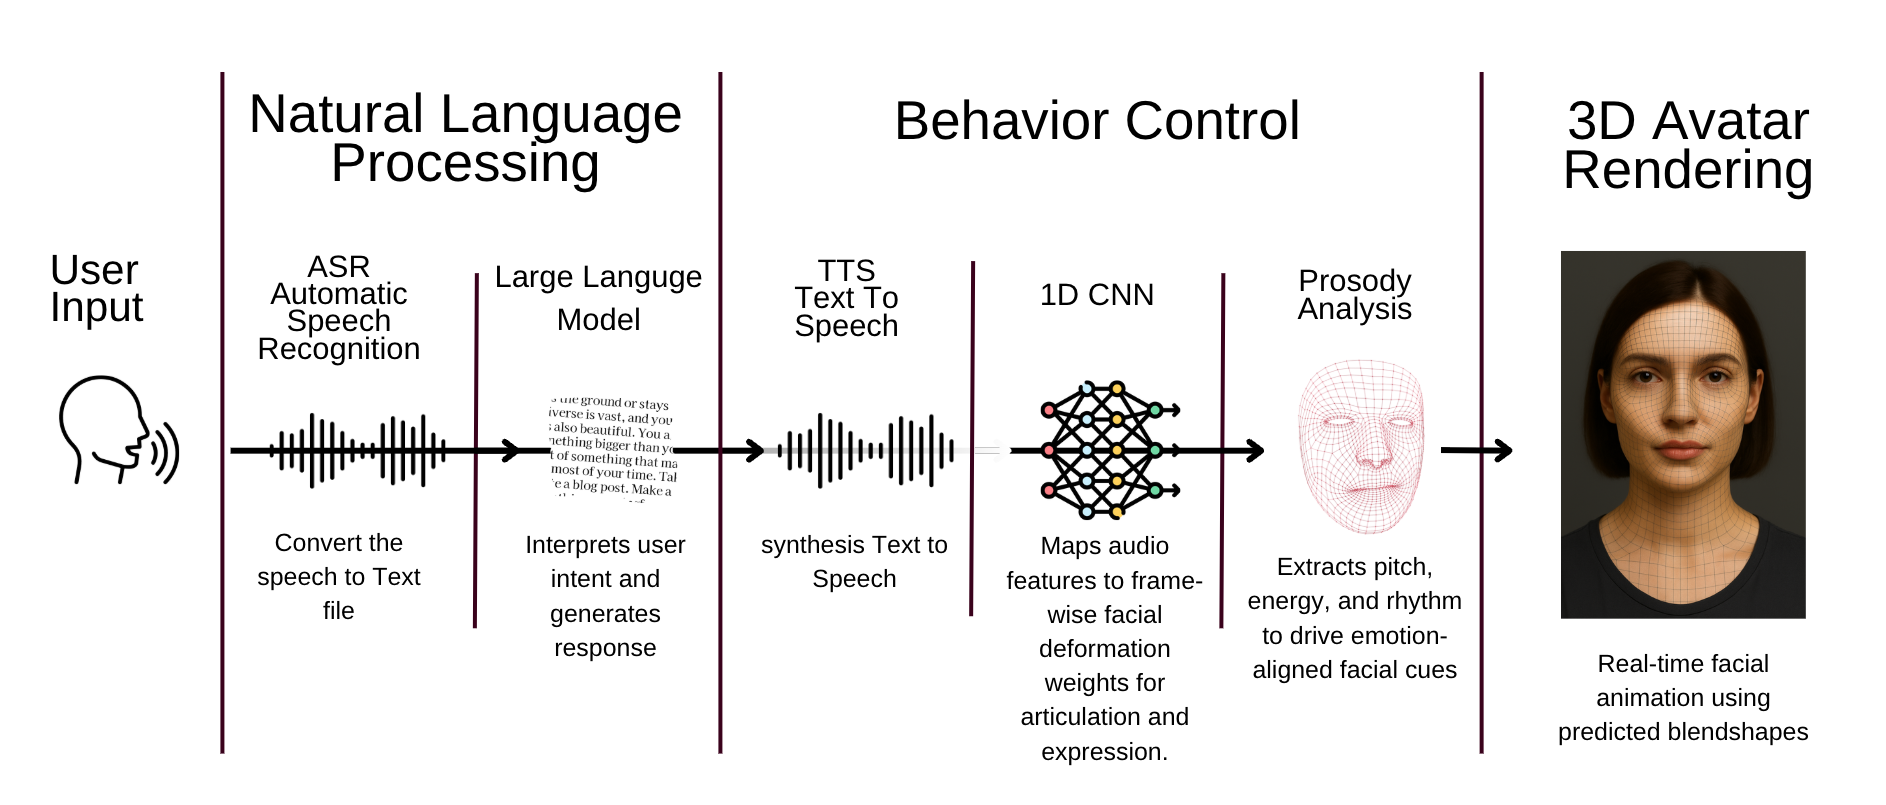
\includegraphics[width=0.85\textwidth]{s.png}
\caption{1D CNN architecture for audio-to-blendshape regression. Log-Mel features are processed through convolutional layers to capture temporal patterns and are mapped to frame-wise blendshape weights for real-time facial animation.}
\label{fig:model-architecture}
\end{figure}

\begin{itemize}
  \item \textbf{Automatic Speech Recognition (ASR):} Converts audio input to structured text using models like OpenAI Whisper, while retaining prosodic features such as pitch and rhythm.
  
  \item \textbf{Large Language Model (LLM):} The transcribed text is processed by an LLM (e.g., GPT-4), which interprets intent, maintains context, and generates responses with semantic and pragmatic depth.
  
  \item \textbf{Text-to-Speech (TTS):} The textual response is vocalized using expressive TTS systems (e.g., Coqui, ElevenLabs), generating human-like speech with controllable prosody and emotional tone.
  
  \item \textbf{Facial Animation \& Blendshape Generation:} In parallel with TTS, the synthesized audio is used to predict blendshape sequences for facial expression animation.
  
  \item \textbf{3D Avatar Rendering:} A rigged avatar (e.g., MetaHuman or Audio2Face) animates in real time using the predicted blendshape weights, producing synchronized lip-sync and micro-expressions.
\end{itemize}

\subsection{Behavior Control Module}

At the core of expressive synthesis lies the blendshape regressor, which maps audio features to facial motion through a dual-stream architecture:

\begin{itemize}
  \item \textbf{Articulatory Stream:} Processes log-Mel spectrograms to extract phonetic content and drive lip and jaw movements. A series of 1D convolutional layers capture local temporal patterns critical to articulation.
  
  \item \textbf{Prosodic Stream:} Analyzes pitch, energy, and timing to infer expressive behaviors—such as eyebrow raises, eye blinks, or subtle nods—that signal affect, emphasis, and engagement.
\end{itemize}

The two streams are fused at a joint representation layer and regressed to frame-wise blendshape vectors, enabling the synthesis of temporally aligned, emotionally expressive facial motion.

\subsection{Embodied, Synchronized Output}

The final outputs—speech and facial animation—are rendered in synchrony, resulting in virtual human responses that are:

\begin{itemize}
  \item \textbf{Verbal:} Coherent, context-aware spoken dialogue
  \item \textbf{Visual:} Expressive, phoneme-accurate facial motion
  \item \textbf{Temporal:} Smooth and synchronized across modalities
\end{itemize}

This multimodal coordination allows virtual humans to express not only linguistic meaning but also emotional nuance and social intent, bridging the gap between human communication and machine interaction.


\section{Conclusion and Future Work}

This paper presented a multimodal framework for real-time virtual human interaction, integrating audio-driven facial animation with conversational intelligence. The proposed system combines automatic speech recognition, large language models, and expressive text-to-speech with a dual-stream behavior control module that maps prosodic and phonetic features to facial blendshape parameters. By capturing both the linguistic content and expressive tone of speech, the system enables synchronized verbal and non-verbal responses through a 3D avatar, enhancing naturalness and user engagement in human-computer interaction.

Looking ahead, several directions remain open for expansion. Emotion-aware modeling could enhance affective realism, while integrating gaze and gesture would further enrich the agent's expressive bandwidth. Support for multilingual and culturally adaptive interaction would broaden applicability, and personalization via avatar and voice cloning could increase user relatability. These advancements hold promise across domains such as education, healthcare, entertainment, and accessibility—positioning virtual humans as expressive, intelligent interfaces in the next generation of digital systems.








%
% ---- Bibliography ----
%
% BibTeX users should specify bibliography style 'splncs04'.
% References will then be sorted and formatted in the correct style.
%
% \bibliographystyle{splncs04}
% \bibliography{mybibliography}
%
\begin{thebibliography}{8}

\bibitem{ref_virtualhuman_survey}
Bevan, C., Green, D., Farmer, H., Rose, M., Cater, K.: The interaction design of 3D virtual humans: A survey. ACM Computing Surveys (CSUR) \textbf{55}(4), 1–38 (2022). \doi{10.1145/3491056}

\bibitem{ref_facs}
Ekman, P., Friesen, W.V.: Facial Action Coding System: A Technique for the Measurement of Facial Movement. Consulting Psychologists Press (1978)

\bibitem{ref_multistream}
Richard, A., Robineau, J., Bérar, M., Devillers, L.: Multi-stream end-to-end audio to 3D face generation with emotion conditioning. arXiv preprint \texttt{arXiv:2106.12461} (2021)

\bibitem{ref_affectivehead}
Cowie, R., Douglas-Cowie, E., Savvidou, S., McMahon, E., Sawey, M., Schröder, M.: Multimodal affect: Perceptually evaluating an affective talking head. In: Proc. 4th IEEE Int. Conf. on Multimodal Interfaces, pp. 21–26. IEEE (2002). \doi{10.1109/ICMI.2002.1166981}

\bibitem{ref_rag}
Lewis, P., Perez, E., Piktus, A., Petroni, F., Karpukhin, V., Goyal, N., Küttler, H., Lewis, M., Yih, W.T., Rocktäschel, T., Riedel, S.: Retrieval-Augmented Generation for Knowledge-Intensive NLP Tasks. In: Advances in Neural Information Processing Systems (NeurIPS), vol. 33, pp. 9459–9474 (2020)

\bibitem{ref_whisper}
Radford, A., Kim, J.W., Xu, T., et al.: Whisper: Robust speech recognition via large-scale weak supervision. OpenAI (2023). \url{https://openai.com/research/whisper}

\bibitem{ref_voca}
Cudeiro, D., Otaduy, M.A., Black, M.J., Pons-Moll, G.: Capture, Learning, and Synthesis of 3D Speaking Styles. In: Proc. IEEE/CVF Conf. on Computer Vision and Pattern Recognition (CVPR), pp. 10101–10111 (2019). \doi{10.1109/CVPR.2019.01034}

\bibitem{ref_emoface}
Liu, Y., Chai, M., Xu, M., Kiran, T.R., Narayana, M., Al-Halah, Z.: EmoFace: Emotion-Aware Audio-Driven Facial Animation. In: Proc. IEEE/CVF Conf. on Computer Vision and Pattern Recognition (CVPR), pp. 28455–28465 (2024). \doi{10.1109/CVPR.2024.00412}

\end{thebibliography}
\end{document}
